% pdflatex rapport.tex
%----------------------------------------------------------------------------------------
%	PACKAGES AND OTHER DOCUMENT CONFIGURATIONS
%----------------------------------------------------------------------------------------

\documentclass[13pt]{article}
\usepackage[francais]{babel}
\usepackage[utf8x]{inputenc}
\usepackage{amsmath}
\usepackage{graphicx}
\usepackage{float}
\usepackage{titlesec}
\usepackage{subcaption}
\usepackage{listings}
\usepackage{hyperref}
\hypersetup{%
    pdfborder = {0 0 0}
}
\usepackage[colorinlistoftodos]{todonotes}
\setlength{\parindent}{3em}
\setcounter{secnumdepth}{4}
\titleformat{\paragraph}
{\normalfont\normalsize\bfseries}{\theparagraph}{1em}{}
\titlespacing*{\paragraph}
{0pt}{3.25ex plus 1ex minus .2ex}{1.5ex plus .2ex}
\begin{document}
\lstset{language=Pascal} 
\begin{titlepage}

\newcommand{\HRule}{\rule{\linewidth}{0.5mm}} % Defines a new command for the horizontal lines, change thickness here

\center % Center everything on the page
 
%----------------------------------------------------------------------------------------
%	HEADING SECTIONS
%----------------------------------------------------------------------------------------

\textsc{\LARGE EISTI}\\[1.5cm] % Name of your university/college
\textsc{\Large Mini-Projet : Application des tris}\\[0.5cm] % Major heading such as course name
\textsc{\large Algorithmique et programmation procédurale}\\[0.5cm] % Minor heading such as course title

%----------------------------------------------------------------------------------------
%	TITLE SECTION
%----------------------------------------------------------------------------------------

\HRule \\[0.4cm]
{ \huge \bfseries  Rapport de Projet}\\[0.4cm] % Title of your document
\HRule \\[1cm]
 
%----------------------------------------------------------------------------------------
%	AUTHOR SECTION
%----------------------------------------------------------------------------------------

\Large
David \textsc{RIGAUX}\\[0.5cm]
Maxime \textsc{LUNDQUIST}\\[1cm]

%----------------------------------------------------------------------------------------
%	DATE SECTION
%----------------------------------------------------------------------------------------

{\large \today}\\[1cm] % Date, change the \today to a set date if you want to be precise

%----------------------------------------------------------------------------------------
%	LOGO SECTION
%----------------------------------------------------------------------------------------


\includegraphics{Logo_EISTI.png}\\[1cm] % Include a department/university logo - this will require the graphicx package
 
%----------------------------------------------------------------------------------------

\vfill % Fill the rest of the page with whitespace

\end{titlepage}

\tableofcontents
\newpage

\section{Introduction}

Tout d'abord, ce mini-projet avait pour but d'écrire deux programmes.
Le premier consistait à calculer combien de réincarnations devrait faire une personne avant d'atteindre le nirvana en fonction de son prénom selon le grand sage Shakâchâraya. Ce nombre est codé dans son prénom. L'utilisateur doit avoir la possibilité d'entrer un certain nombre de prénoms tout en majuscule, faisant abstraction des accents et des cédilles   et le programme doit renvoyer les prénoms dans l'ordre croissant selon leur avancement spirituel.
Le second, quant à lui, consistait à faire un programme permettant de calculer le classement final d'un tournoi de football tel celui de Trifouillis-les-Oies. Pour être plus précis, chaque équipe du tournoi joue exactement une fois contre toutes les autres équipes. Il faut savoir qu’ une victoire compte 3 points pour les gagnants, et 0 pour les perdants. Un nul compte 1 point par équipe. Le classement est ensuite établi à la fin de tous les matchs grâce au score entré par l'utilisateur suivant plusieurs règles de classement.

\section{Notions préliminaires}
\subsection{Le tri rapide}
Le tri rapide consiste à partitionner le tableau en deux parties séparées par un pivot de telle sorte que :
\begin{itemize}
\item Les éléments de la partie gauche soient tous inférieurs ou égaux à ce pivot
\item Et ceux de la partie droite soient tous supérieurs à ce pivot
\end{itemize}
Puis, appliquer (récursivement) un tri rapide sur ces deux parties. Le tri rapide a été fait en cours donc nous avons repris le code réalisé en classe.
\section{Réalisation du projet}
Dans un premier temps, nous avions à savoir comment fonctionne chacun des deux programmes, leurs mécanismes, et surtout par où commencer. Après avoir compris le but des sujets il fallait ensuite s'imaginer comment les coder, et toutes les précautions à prendre. Nous avons donc fait plusieurs schémas sur papiers pour nous aider à visualiser comment nous allions procéder à la programmation. Nous avons choisi de faire un programme contenant les deux parties, chacun codé en Unit.
\subsection{Réincarnation}
\subsubsection*{Calcul du nombre de réincarnations selon le critère du grand sage Shakâchâraya}
Dans la partie \emph{Réincarnation} nous devions faire en sorte que l'utilisateur puisse entrer un nombre fini de prénoms tous en majuscules. Nous demandons donc à l'utilisateur d'entrer le nombre de prénoms qu'ils souhaitent utiliser. Grâce à ce nombre, nous pouvons ainsi définir la longueur du tableau contenant les noms, qui est un tableau dynamique de strings, et ensuite lui demander de les entrer un par un. Pour éviter d'entrer l'alphabet complet dans le code et créer alors 26 variables, nous avons choisi d'utiliser le code ASCII de chaque caractère pour pouvoir établir un ordre et en même temps vérifier qu'il ne s'agit exclusivement que de lettres en majuscules. 

\begin{figure}[H]
\centering
\begin{subfigure}[H]{.5\textwidth}
  \centering
  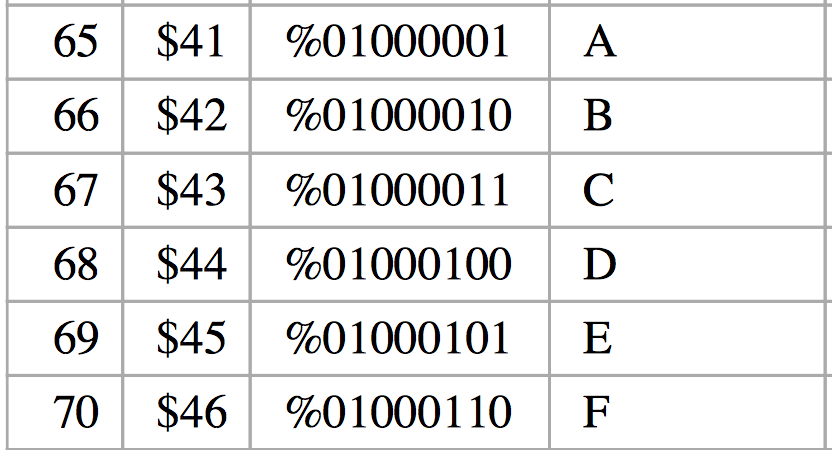
\includegraphics[width=0.8\textwidth]{A.png}
  \caption{Début de l'alphabet en majuscule}
\end{subfigure}%
\begin{subfigure}[H]{.5\textwidth}
  \centering
  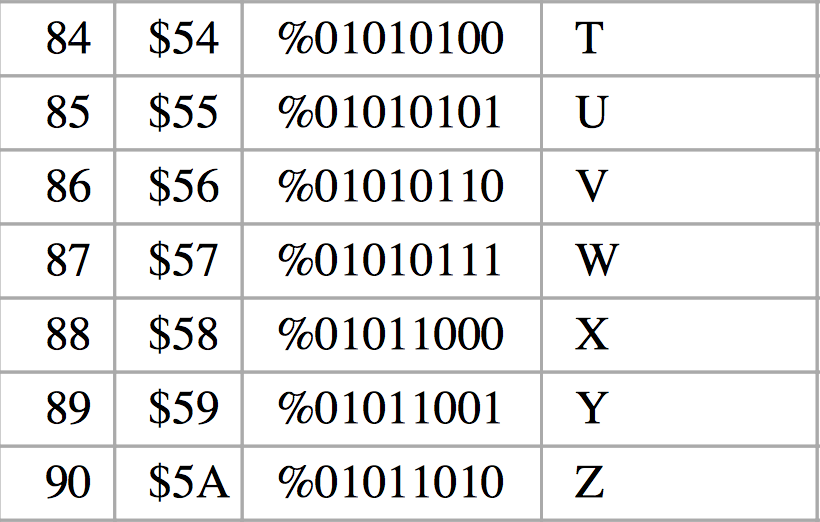
\includegraphics[width=0.8\textwidth]{Z.png}
  \caption{Fin de l'alphabet en majuscule}
\end{subfigure}
\end{figure}
En effet, on remarque que \emph{"A"} étant la première lettre de l'alphabet à comme code ASCII le nombre 65, et \emph{"Z"} le code 90. Ainsi, nous avons introduit une boucle qui vérifie que toutes les lettres des prénoms sont bien dans l'intervalle [65;90]. Si ce n'est pas le cas, après avoir entré tous les prénoms, un message d'erreur s'affiche et nous indique quel prénom n'est pas exclusivement en majuscule et quitte le programme. Dans le cas où il y en a plusieurs, le premier entré avec un caractère autre qu'une majuscule est affichée dans le message d'erreur. En faisant le test pour la majuscule, nous en avons aussi profité pour calculer la somme de toutes les lettres de chaque prénom selon l'ordre alphabétique. Pour cela nous avons utiliser la fonction \emph{ord()}, qui permet de ressortir la valeur en ASCII d'une lettre, et de cette valeur ressortis nous soustrayions aussitôt 64, car cela nous permet d'avoir la position des lettres dans l'alphabet dans l'intervalle [1;26]. Nous ajoutons donc la valeur de toutes les lettres du prénom pour avoir la valeur totale du prénom. \\
D'après l'énoncé nous devons ensuite multiplier cette valeur par \emph{47} puis lui ajouter \emph{19}. La valeur que nous avons ensuite doit être décomposé chiffre par chiffre c'est-à-dire par exemple avec le nombre 2705, nous devons le décomposer ainsi : \emph{2 7 0 5}, et ajouter touts les chiffres l'un avec l'autre. Pour procéder à la décomposition du nombre, nous avons utilisé la procédure \emph{IntToStr} qui nous permet de convertir une chaîne de caractères (\emph{STRING}) en entier (\emph{INTEGER}). En effet, sachant qu'une chaîne de caractères peut être manipuler comme un tableau de caractères nous pouvons ainsi prendre élément par élément et les ajoutant les uns avec les autres en appliquant pour chaque lettre \emph{StrToInt}, ce qui nous donne finalement le nombre de réincarnations du prénom pour atteindre le nirvana selon le grand sage Shakâchâraya. Ces valeurs sont ensuite stockées dans un tableau ayant les mêmes caractéristiques que le tableau dynamique contenant les prénoms, mais cette fois ce tableau permet de stocker des entiers. Pour s'y retrouver parmi les valeurs, elles ont la même position dans le tableau que le prénom correspondant dans le premier tableau, ce qui facilite la tâche du tri.
\subsubsection*{Tri selon l'avancement spirituel des prénoms}
Pour effectuer le tri des prénoms nous nous sommes mis tout d’abord d'accord sur le que de tri utiliser et nous avons choisis le tri rapide. Pour appliquer le tri rapide à ce programme, quand le tri change une valeur il faut bien penser à changer également l'ordre des prénoms dans le tableau correspondant, donc à créer des variables en plus pour le pivot des prénoms, mais aussi pour le changement de cases donc créer une variable de substitution.
Après avoir fait tous les changements adéquats, vos prénoms sont alors triés selon leur avancement spirituel.\\
\\
\par
Il faut maintenant afficher le résultat comme écrit dans le rapport. Pour faire cela, il suffit de manipuler la fonction \emph{Write} et \emph{WriteLN}. C'est-à-dire introduire une boucle \emph{FOR} qui permet de parcourir la longueur du tableau : 
\begin{lstlisting}[language=Pascal]
FOR i := 0 to x-1 DO BEGIN
    if (i = (x-1)) then WRITELN(str[i],' (',inte[i],')')
    ELSE WRITE(str[i],' (',inte[i],') - ');
  END;
 \end{lstlisting}

  
\subsection{Tournoi de football}
\subsubsection*{Entré des noms des équipes et des résultats}
Pour créer le classement du tournoi de foot comme demandé, nous avons choisi de créer un \emph{RECORD} qui comprend 4 tableaux dynamiques (un de chaîne de caractères et trois d'entiers), ils ont tous la même longueur. Le tableau de chaîne de caractères sert à stocker le nom des équipes participantes, un des tableaux d'entier permet de stocker les points de l'équipe et les deux autres sont les tableaux permettant de stocker les buts marqués d'une part et ceux encaissés dans le tableau restant. \\
Pour pouvoir initialiser tous les tableaux, l'utilisateur doit entrer le nombre d'équipes participantes au tournoi. À ce moment-là, le tableau réservé pour les noms d'équipes est initialisé et grâce à une boucle \emph{FOR} l'utilisateur peut ensuite entrer le nom de chaque équipe l'un à la suite de l'autre. Pour s'y retrouver entre les résultats des matchs, nous avons fait en sorte de nousorganiser comme pour le programme sur la réincarnation, c'est-à-dire tous les résultats d'une équipe ont le même indice que le nom lui-même. Après avoir entré tous les noms des équipes, il ne reste plus qu'à entrer les résultats du match. Pour cela nous avons créé une double boucle \emph{FOR} permettant de faire que toutes les équipes se rencontrent une fois et qu'une seule fois. Quand l'utilisateur a entré les résultats d'un match, l'algorithme compare les deux résultats, et en déduit qui est le vainqueur de la rencontre. Il ajoute ensuite les points qu'il faut à l'équipe concernée. Donc 3 points en plus sur la valeur qu'il a déjà et ajoute également le nombre de buts marqué et encaissé. À partir de ce point, quand l'utilisateur a fini d'entrer tous les résultats des matchs, le tri entre finalement en action.
\subsubsection*{Tris et classement des résultats}
Maintenant que touts les résultats ont été entrés dans les tableaux correspondants, nous devons trier les résultats de façon décroissante pour que l'équipe ayant le plus de points soit au début des tableaux et l'équipe avec le moins de points à la fin des tableaux. Pour procéder au tri, nous avons pris la même méthode que pour la réincarnation, c'est-à-dire un tri rapide, mais cette fois-ci au lieu de traiter deux tableaux nous en traitons quatre, il faut donc créer les variables qu'il faut en plus et juste changer deux signes dans une double boucle \emph{While} et le tri rapide dans l'ordre décroissant est fait.
\\
Dorénavant ayant trié les tableaux, il arrive que des fois deux équipes aient le même nombre de points, c'est pour cela qu'il y a certains critères à respecter pour départager les deux équipes. En effet s’ il y a égalité en nombre de points entre deux équipes, nous devons alors nous intéresser à la différence de nombre de buts marqués et encaissés, si cela ne suffit toujours pas alors nous regardons le nombre de buts marqué et finalement s’ il y a toujours égalité nous les classons selon l'ordre alphabétique. Pour comparer la différence de buts de deux équipes, nous prenons le nombre de buts marqués et nous soustrayions le nombre de buts encaissé par une équipe et nous faisons ensuite une comparaison de la différence. Le procédé est le même pour comparer le nombre de buts marqués sauf que nous ne faisons pas la soustraction des buts encaissés. Et finalement pour l'ordre alphabétique, nous comparons l'ordre alphabétique des lettres des deux équipes une par une. Pour faire cela, nous avons utilisé la même méthode que pour la partie d'avant avec les valeurs des lettres en ASCII. Cependant, ce à quoi il fallait penser dans cette partie était le cas où le nom des équipes n’ est pas exclusivement écrit en majuscule ou minuscule donc il fallait faire un test pour voir s'il faisait partie de l'ensemble des majuscules ou dans l'ensemble des minuscules.

\begin{figure}[H]
\centering
\begin{subfigure}[H]{.5\textwidth}
  \centering
  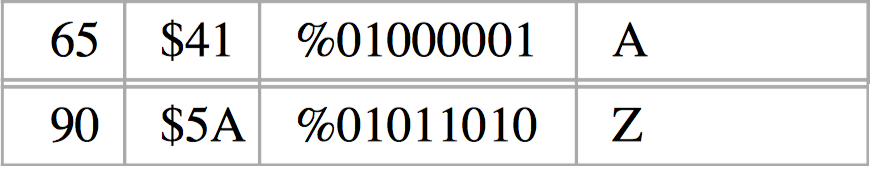
\includegraphics[width=0.8\textwidth]{majaz.png}
\caption{Alphabet en majuscule [65;90]}
\end{subfigure}%
\begin{subfigure}[H]{.5\textwidth}
  \centering
  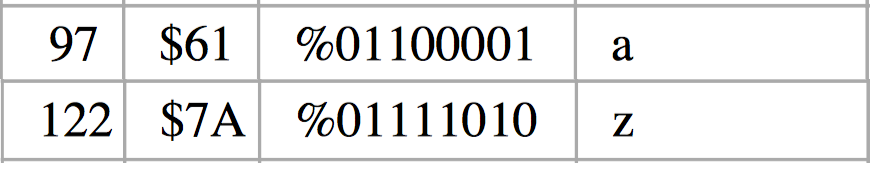
\includegraphics[width=0.8\textwidth]{minaz.png}
\caption{Alphabet en minuscule [97;122]}
\end{subfigure}
\end{figure}
S’ il s'agit de majuscules alors il faut qu'on soustraie 64 à la valeur obtenue grâce à \emph{ord()} et soustraire 96 s'il s'agit d'une minuscule.
Pour tous les cas où il faut effectivement changer l'ordre, nous précédons comme dans le tri rapide où nous passons par une variable de substitution, mais il faut bien penser à changer l'ordre dans les quatre tableaux.\\
Maintenant que tout ce qui est classement est fait, il ne nous reste plus qu'à nous occuper de la mise en forme du tableau qui affiche à l'utilisateur le classement final du tournoi.
\subsubsection{Mise en forme du classement}
Comme le nom de chaque équipe est de longueur différente, il fallait que nous trouvions une formule permettant de calculer le nombre d'espaces qu'il fallait mettre sur chaque nom pour que tout soit aligné à l'espace près. Pour faire cela, nous avons fait une boucle \emph{FOR} qui parcourt tout le tableau de noms et regarde la longueur de chaque nom d'équipe à l'aide de \emph{length}, qui permet de ressortir la taille d'un tableau. En faisant cela, nous cherchons à trouver la longueur maximale des noms. Après l'avoir trouvé, commence les maths et l'utilisation de la formule. Pour trouver cette formule, nous avons dû faire sur papier cadrer pour calculer sur des exemples les espaces qu'il nous fallait pour faire une mise en forme convenable. Commençons par le commencement, pour le titre "\emph{Équipe}", nous remarquons qu'il comporte 7 lettres, nous faisons donc la différence de lettres entre le nom le plus long et nous ajoutons le nombre d'espace correspondant à la différence avec une marge de deux espaces pour pas que ce ne soit trop collé. Grâce à cela nous avons alors la position des titres \emph{Points} et \emph{Buts}. Nous appliquons la même méthode à tous les autres noms, en calculant la différence des lettres et en ajoutant le nombre de blancs correspondant, mais il existe deux cas de figure où il faut procéder différemment. En effet, si un deuxième nom à la même longueur alors nous n'ajoutons que deux espaces derrière ce nom. Et le deuxième cas de figure survient si la différence de lettres est de 1, sachant que nous prenons une marge de deux espaces, dans ce cas s’ il faut que l'on ajoute trois espaces derrière ce nom-là. Pour ce qui est des l'alignement du nombre de points et de buts cela peut se faire, comme nous avons faits, en jouant avec les espaces dans les \emph{WRITE}.

\begin{figure}[H]
\centering
\begin{subfigure}[H]{.5\textwidth}
  \centering
 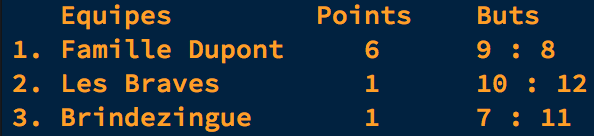
\includegraphics[width=0.8\textwidth]{ex1.png}
\caption{Premier exemple}
\end{subfigure}%
\begin{subfigure}[H]{.5\textwidth}
  \centering
  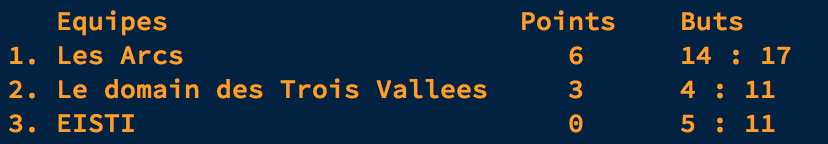
\includegraphics[width=0.9\textwidth]{ex2.png}
\caption{Deuxième exemple}
\end{subfigure}
\end{figure}

Voilà ce que nous avons quand la mise en forme est bien faite comme décrit au-dessus.
\section{Bilans Personnels}
\subsection{Maxime Lundquist}

J'ai fait le début des deux programmes et pour la réincarnation j'ai eu du mal à comprendre comment utiliser un string (je ne l'avais jamais utilisé avant) et aussi l'instruction ord, vu qu'elle est toute nouvelle.
Pour le tournoi, j'ai fait les entrées de noms d'équipes. J'ai aussi aidé David à faire l'entrée des scores, car on ne voyait pas comment attribuer les scores à chacune des équipes et surtout pour le classement final pour les comptages de point selon le résultat du match. 
\subsection{David Rigaux}
Pour ma part dans le projet je me suis occupé essentiellement des manipulations de tableaux. Dans la partie de la réincarnation, je me suis chargé des calculs à faire avec l'aide de Maxime. Durant ce projet j'ai appris à utiliser les codes ASCII dans un algorithme et on se rend compte que c'est très utile et facile. Le programme de la réincarnation était relativement simple cependant au début j'ai eu du mal à assimiler le fait qu'il fallait créer des variables en plus pour le pivot des noms, mais une fois intégré dans le code il marchait très bien. Comme Maxime à dit précédemment, pour faire le programme qui créer le classement du tournoi au début on à eu du mal avec les indices des tableaux. J'ai toujours eu un peu de mal avec les \emph{RECORD} donc l'utiliser ici ne m'a fait que du bien et je commence à beaucoup plus l'assimiler. J'ai également fait la sortie du classement. À certains moments j'avais des erreurs lors de l'utilisation du programme, mais avec Maxime nous avons regardé le code et finalement le plus souvent il ne s'agit que d'erreurs d'indice. En effet, il y avait tellement tableaux qu'à certains moments on s'y perdait. Mais ce mini-projet m'a permis à accentuer quelques capacités en algorithmique, ce qui est très satisfaisant.
\section{Conclusion}
Ce mini-projet d'application de tris nous permet de voir en quel cas on pourrait avoir à utiliser les tris de tableaux et comment l'implémenter selon le cas de figure, ce qui est très intéressant. Avoir travaillé avec pleins de tableaux, des \emph{RECORD} et avoir découvert une nouvelle structure (ord) cela nous a permis à apprendre certaines notions, mais surtout à améliorer nos capacités de programmation.
\end{document}